\documentclass[dvisvgm,tikz,border=4pt]{standalone}\usepackage{amsmath,amssymb}
\usetikzlibrary{arrows.meta,decorations.markings,backgrounds,cd,calc}
\colorlet{c1}{blue!70!black}\colorlet{c2}{red!70!black}\colorlet{c3}{green!45!black}
\tikzset{
 ->-/.style={decoration={markings,mark=at position .55 with {\arrow{Stealth[length=2.4mm]}}},postaction={decorate}},
 ->>-/.style={decoration={markings,mark=at position .5 with {\arrow{Stealth[length=2.4mm]}},mark=at position .6 with {\arrow{Stealth[length=2.4mm]}}},postaction={decorate}},
 every picture/.append style={show background rectangle, background rectangle/.style={fill=white}}
}

\begin{document}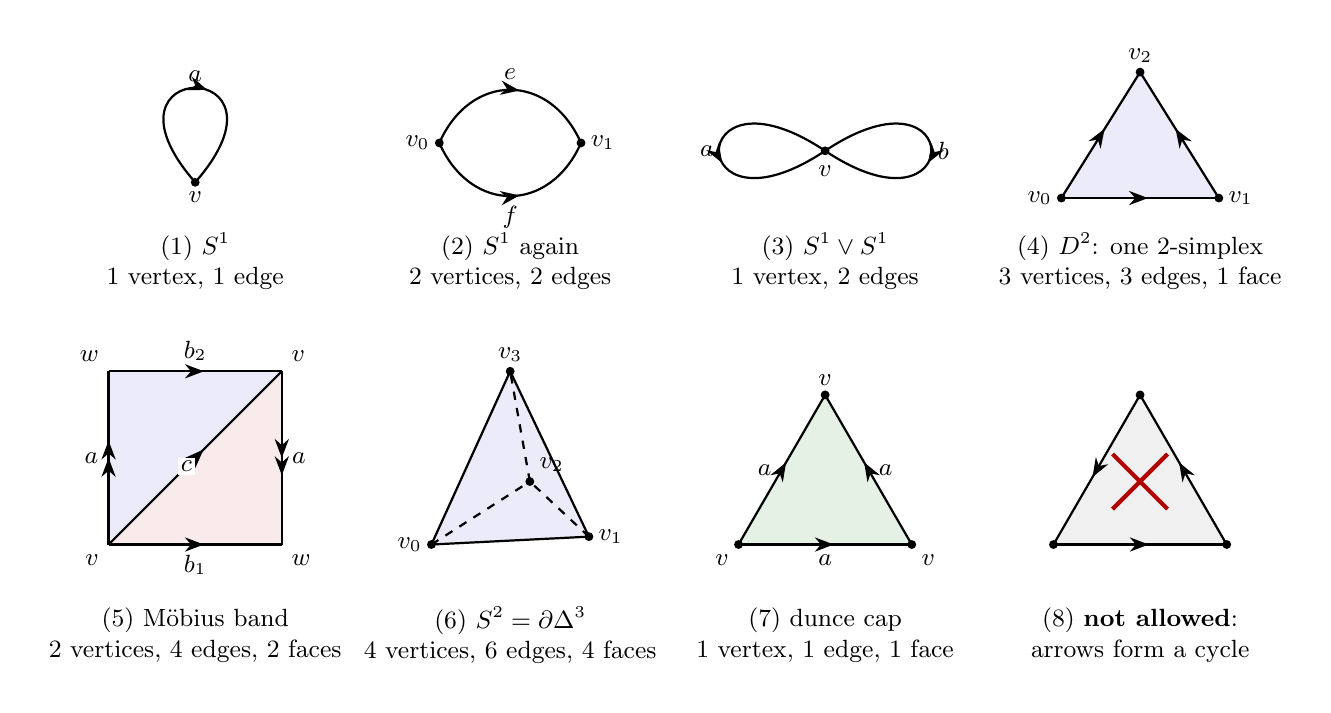
\begin{tikzpicture}[every node/.style={font=\small}]
% 1: S^1, one vertex
\begin{scope}
\draw[thick,->-] (0,0) .. controls (-1.4,1.6) and (1.4,1.6) .. (0,0);
\fill (0,0) circle(1.6pt) node[below]{$v$}; \node at (0,1.35){$a$};
\node[align=center] at (0,-1){(1) $S^1$\\ $1$ vertex, $1$ edge};
\end{scope}
% 2: S^1, two vertices
\begin{scope}[xshift=4cm]
\draw[thick,->-] (-0.9,0.5) .. controls (-0.5,1.4) and (0.5,1.4) .. (0.9,0.5) node[pos=.5,above]{$e$};
\draw[thick,->-] (-0.9,0.5) .. controls (-0.5,-0.4) and (0.5,-0.4) .. (0.9,0.5) node[pos=.5,below]{$f$};
\fill (-0.9,0.5) circle(1.6pt) node[left]{$v_0$}; \fill (0.9,0.5) circle(1.6pt) node[right]{$v_1$};
\node[align=center] at (0,-1){(2) $S^1$ again\\ $2$ vertices, $2$ edges};
\end{scope}
% 3: S^1 v S^1
\begin{scope}[xshift=8cm]
\draw[thick,->-] (0,0.4) .. controls (-1.8,1.6) and (-1.8,-0.8) .. (0,0.4);
\draw[thick,->-] (0,0.4) .. controls (1.8,1.6) and (1.8,-0.8) .. (0,0.4);
\fill (0,0.4) circle(1.6pt) node[below=2pt]{$v$}; \node at (-1.5,0.4){$a$}; \node at (1.5,0.4){$b$};
\node[align=center] at (0,-1){(3) $S^1\vee S^1$\\ $1$ vertex, $2$ edges};
\end{scope}
% 4: disk
\begin{scope}[xshift=12cm]
\coordinate (A) at (-1,-0.2); \coordinate (B) at (1,-0.2); \coordinate (C) at (0,1.4);
\fill[c1!8] (A)--(B)--(C)--cycle;
\draw[thick,->-] (A)--(B); \draw[thick,->-] (B)--(C); \draw[thick,->-] (A)--(C);
\fill (A) circle(1.6pt) node[left]{$v_0$}; \fill (B) circle(1.6pt) node[right]{$v_1$}; \fill (C) circle(1.6pt) node[above]{$v_2$};
\node[align=center] at (0,-1){(4) $D^2$: one $2$-simplex\\ $3$ vertices, $3$ edges, $1$ face};
\end{scope}
% 5: Mobius band
\begin{scope}[yshift=-4.6cm,xshift=-1.1cm]
\fill[c1!8] (0,0)--(0,2.2)--(2.2,2.2)--cycle; \fill[c2!8] (0,0)--(2.2,0)--(2.2,2.2)--cycle;
\draw[thick,->-] (0,0)--(2.2,0) node[midway,below]{$b_1$};
\draw[thick,->-] (0,2.2)--(2.2,2.2) node[midway,above]{$b_2$};
\draw[thick,->>-] (0,0)--(0,2.2) node[midway,left]{$a$};
\draw[thick,->>-] (2.2,2.2)--(2.2,0) node[midway,right]{$a$};
\draw[thick,->-] (0,0)--(2.2,2.2) node[pos=.45,fill=white,inner sep=1pt]{$c$};
\node[below left] at (0,0){$v$};\node[below right] at (2.2,0){$w$};\node[above left] at (0,2.2){$w$};\node[above right] at (2.2,2.2){$v$};
\node[align=center] at (1.1,-1.15){(5) Möbius band\\ $2$ vertices, $4$ edges, $2$ faces};
\end{scope}
% 6: boundary of tetrahedron
\begin{scope}[yshift=-4.6cm,xshift=4cm]
\coordinate (P0) at (-1,0); \coordinate (P1) at (1,0.1); \coordinate (P2) at (0.25,0.8); \coordinate (P3) at (0,2.2);
\fill[c1!8] (P0)--(P1)--(P3)--cycle;
\draw[thick,dashed] (P0)--(P2) (P1)--(P2) (P2)--(P3);
\draw[thick] (P0)--(P1)--(P3)--cycle;
\foreach \p/\n/\pos in {P0/v_0/left,P1/v_1/right,P2/v_2/above right,P3/v_3/above}{\fill (\p) circle(1.6pt) node[\pos]{$\n$};}
\node[align=center] at (0,-1.15){(6) $S^2=\partial\Delta^3$\\ $4$ vertices, $6$ edges, $4$ faces};
\end{scope}
% 7: dunce cap
\begin{scope}[yshift=-4.6cm,xshift=8cm]
\coordinate (A) at (-1.1,0); \coordinate (B) at (1.1,0); \coordinate (C) at (0,1.9);
\fill[c3!10] (A)--(B)--(C)--cycle;
\draw[thick,->-] (A)--(B) node[midway,below]{$a$}; \draw[thick,->-] (B)--(C) node[midway,right]{$a$}; \draw[thick,->-] (A)--(C) node[midway,left]{$a$};
\foreach \p in {A,B,C} \fill (\p) circle(1.6pt) node[below]{};
\node[below left] at (A){$v$};\node[below right] at (B){$v$};\node[above] at (C){$v$};
\node[align=center] at (0,-1.15){(7) dunce cap\\ $1$ vertex, $1$ edge, $1$ face};
\end{scope}
% 8: non-example
\begin{scope}[yshift=-4.6cm,xshift=12cm]
\coordinate (A) at (-1.1,0); \coordinate (B) at (1.1,0); \coordinate (C) at (0,1.9);
\fill[gray!12] (A)--(B)--(C)--cycle;
\draw[thick,->-] (A)--(B); \draw[thick,->-] (B)--(C); \draw[thick,->-] (C)--(A);
\foreach \p in {A,B,C} \fill (\p) circle(1.6pt);
\draw[c2,line width=1.5pt] (-0.35,0.45)--(0.35,1.15) (-0.35,1.15)--(0.35,0.45);
\node[align=center] at (0,-1.15){(8) \textbf{not allowed}:\\ arrows form a cycle};
\end{scope}
\end{tikzpicture}\end{document}
